\chapter{Tái hiện thực nghiệm}
\label{chuong:tai-hien}

Chương này tái hiện lại phần phân tích dữ liệu của bài báo. Toàn bộ mã nguồn, số liệu và kết quả được lưu trên GitHub (Phụ lục~A), và mọi con số trong chương đều được sinh ra từ các script ở thư mục \texttt{src/}.

\section{Quy trình tái hiện}
\label{sec:quy-trinh}

Khó khăn lớn nhất là bài báo \textbf{không công bố dữ liệu gốc}. Mục ``Data Availability Statement'' chỉ ghi rằng dữ liệu được cung cấp khi có yêu cầu hợp lý~\cite{kassem2022}. Vì vậy báo cáo tái hiện theo hai hướng bổ sung cho nhau (Hình~\ref{fig:quy-trinh}):
\begin{itemize}
  \item \textbf{Hướng 1 -- Kiểm tra số liệu đã công bố.} Gõ lại 10 bảng số liệu của bài báo, tính lại mọi chỉ số tính lại được từ chính các bảng đó, rồi đối chiếu với số đã in. Hướng này trả lời câu hỏi: \emph{các con số trong bài có nhất quán với nhau không?}
  \item \textbf{Hướng 2 -- Phân tích trên dữ liệu mô phỏng.} Sinh một bộ 314 phiếu khảo sát giả lập, có tương quan, loading và hệ số đúng như bài báo công bố, rồi chạy lại toàn bộ quy trình phân tích. Hướng này trả lời câu hỏi: \emph{nếu dữ liệu thật có cấu trúc như bài báo mô tả, thì quy trình chuẩn sẽ cho ra kết quả như thế nào?}
\end{itemize}

\begin{figure}[H]
\centering
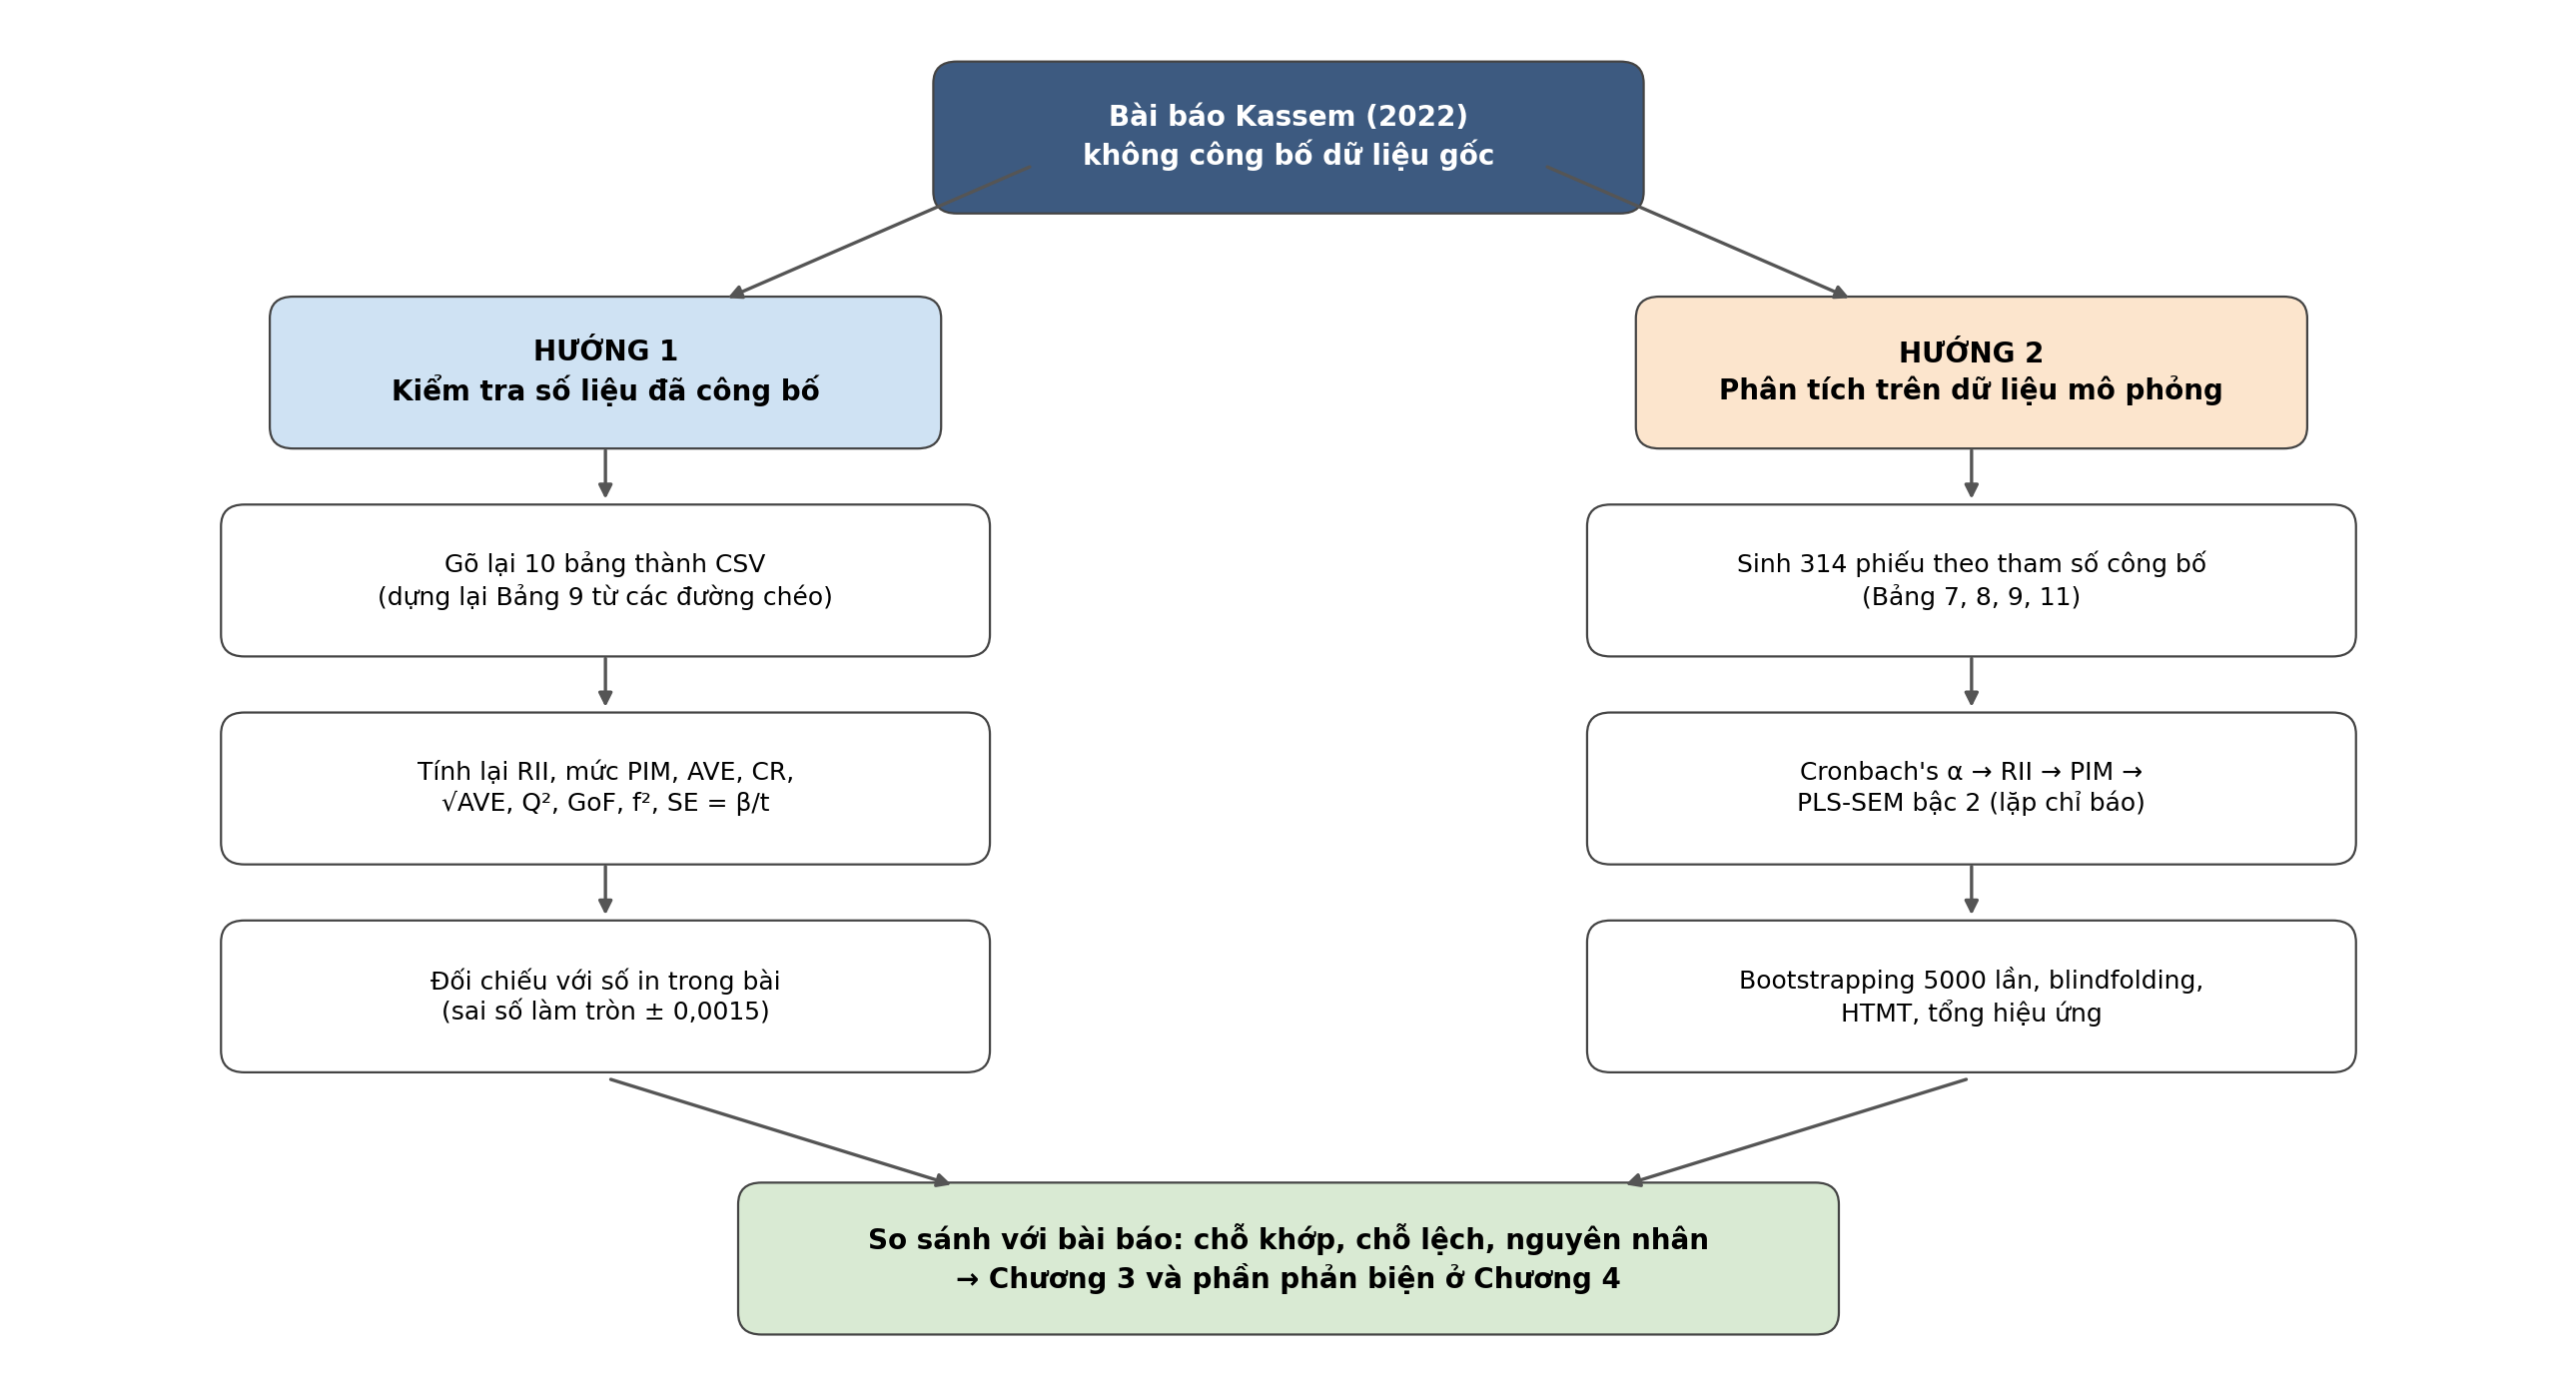
\includegraphics[width=\textwidth]{quy_trinh_tai_hien.png}
\caption{Quy trình tái hiện thực nghiệm theo hai hướng}
\label{fig:quy-trinh}
\end{figure}

\textbf{Công cụ.} Bài báo dùng SPSS v25 và SmartPLS 3, đều là phần mềm thương mại. Báo cáo dùng Python 3 với các thư viện mã nguồn mở numpy, pandas và matplotlib. Thuật toán PLS-SEM, bootstrapping, blindfolding và HTMT được tự cài đặt theo đúng các bước ở mục~\ref{sec:pls-sem}. Để kiểm tra phần cài đặt, mô hình được chạy thử trên một bộ dữ liệu biết trước đáp án: hai biến tiềm ẩn, mỗi biến 4 câu hỏi có loading thật 0,85, hệ số đường dẫn thật 0,6, cỡ mẫu 2000. Kết quả cho loading 0,88--0,89 và hệ số đường dẫn 0,544. Như vậy loading bị ước lượng cao hơn và hệ số đường dẫn thấp hơn giá trị thật, đúng với tính chất đã biết của PLS-SEM~\cite{dijkstra2015}.

\section{Kiểm tra số liệu đã công bố}
\label{sec:kiem-tra}

\subsection{Nhập số liệu}

Mười bảng của bài báo (Bảng 5 tới Bảng 14) được gõ lại thành file CSV. Nhiều bảng trong bản PDF bị lệch cột hoặc lệch hàng, nên phải căn chỉnh lại:
\begin{itemize}
  \item Bảng 5: cột số câu hỏi và cột $\alpha$ bị đẩy xuống một dòng. Căn lại sao cho tổng số câu bằng 51.
  \item Bảng 7: các cột RII tác động và RII xác suất không thẳng hàng với tên rủi ro. Căn lại theo thứ tự dòng, rồi kiểm tra bằng phép nhân ở mục~\ref{sec:kt-rii}.
  \item Bảng 9: ma trận Fornell--Larcker bị in theo từng \emph{đường chéo}. Dòng đầu tiên là đường chéo chính ($\sqrt{AVE}$), dòng thứ hai là đường chéo kế tiếp, v.v. Ma trận được dựng lại thành dạng tam giác dưới $13 \times 13$. Kết quả hợp lý: đường chéo trùng với $\sqrt{AVE}$ tính từ Bảng 8, và ma trận đầy đủ là xác định dương (trị riêng nhỏ nhất bằng 0,092).
  \item Bảng 11: tên các nhóm và các giá trị bị lệch hàng. Ghép lại theo thứ tự chữ cái tiếng Anh của Hình 8 trong bài báo.
\end{itemize}

Bảng~\ref{tab:tong-hop-kiem-tra} tóm tắt kết quả của chín phép kiểm tra. Các mục tiếp theo trình bày chi tiết.

\begin{table}[H]
\centering
\caption{Tổng hợp kết quả kiểm tra số liệu đã công bố}
\label{tab:tong-hop-kiem-tra}
\begin{tabularx}{\textwidth}{@{}clXc@{}}
\toprule
\textbf{TT} & \textbf{Phép kiểm tra} & \textbf{Kết quả} & \textbf{Đánh giá} \\
\midrule
1 & $RII_{tong} = RII_I \times RII_P$ (Bảng 7) & 10/10 dòng khớp, thứ hạng giữ nguyên & Khớp \\
2 & Mức PIM (Bảng 6) so với RII (Bảng 7) & 3/6 rủi ro khớp & Lệch \\
3 & AVE, CR của 13 nhóm từ loading (Bảng 8) & 13/13 khớp & Khớp \\
4 & AVE của biến kết quả EF & 0,494 so với 0,549 & Lệch \\
5 & Fornell--Larcker (Bảng 9) & Nhóm RM không đạt & Lệch \\
6 & Sai số chuẩn suy ra $\beta / t$ (Bảng 11) & Nhỏ bất thường (0,003--0,006) & Nghi vấn \\
7 & $Q^2 = 1 - SSE/SSO$ (Bảng 14) & 3/3 khớp & Khớp \\
8 & GoF (mục 4.3.6e) & Khớp 0,638 nhưng không rõ AVE 0,566 & Nghi vấn \\
9 & $R^2$, $f^2$ so với tương quan ở Bảng 9 & Gần khớp & Khớp \\
\bottomrule
\end{tabularx}
\end{table}

\subsection{RII và ma trận xác suất -- tác động}
\label{sec:kt-rii}

Nhân RII tác động với RII xác suất của 10 rủi ro hàng đầu (công thức~\eqref{eq:rii-tong}) cho ra đúng RII tổng mà bài báo công bố ở cả 10 dòng, với sai lệch không quá 0,0007 do làm tròn. Thứ hạng tính lại cũng giống hệt (Hình~\ref{fig:rii-top10}). Kết quả này xác nhận cách hiểu ở mục~\ref{sec:rii}: $W$ trong công thức~\eqref{eq:rii} là tổng điểm chứ không phải điểm trung bình như bài báo viết.

\begin{figure}[H]
\centering
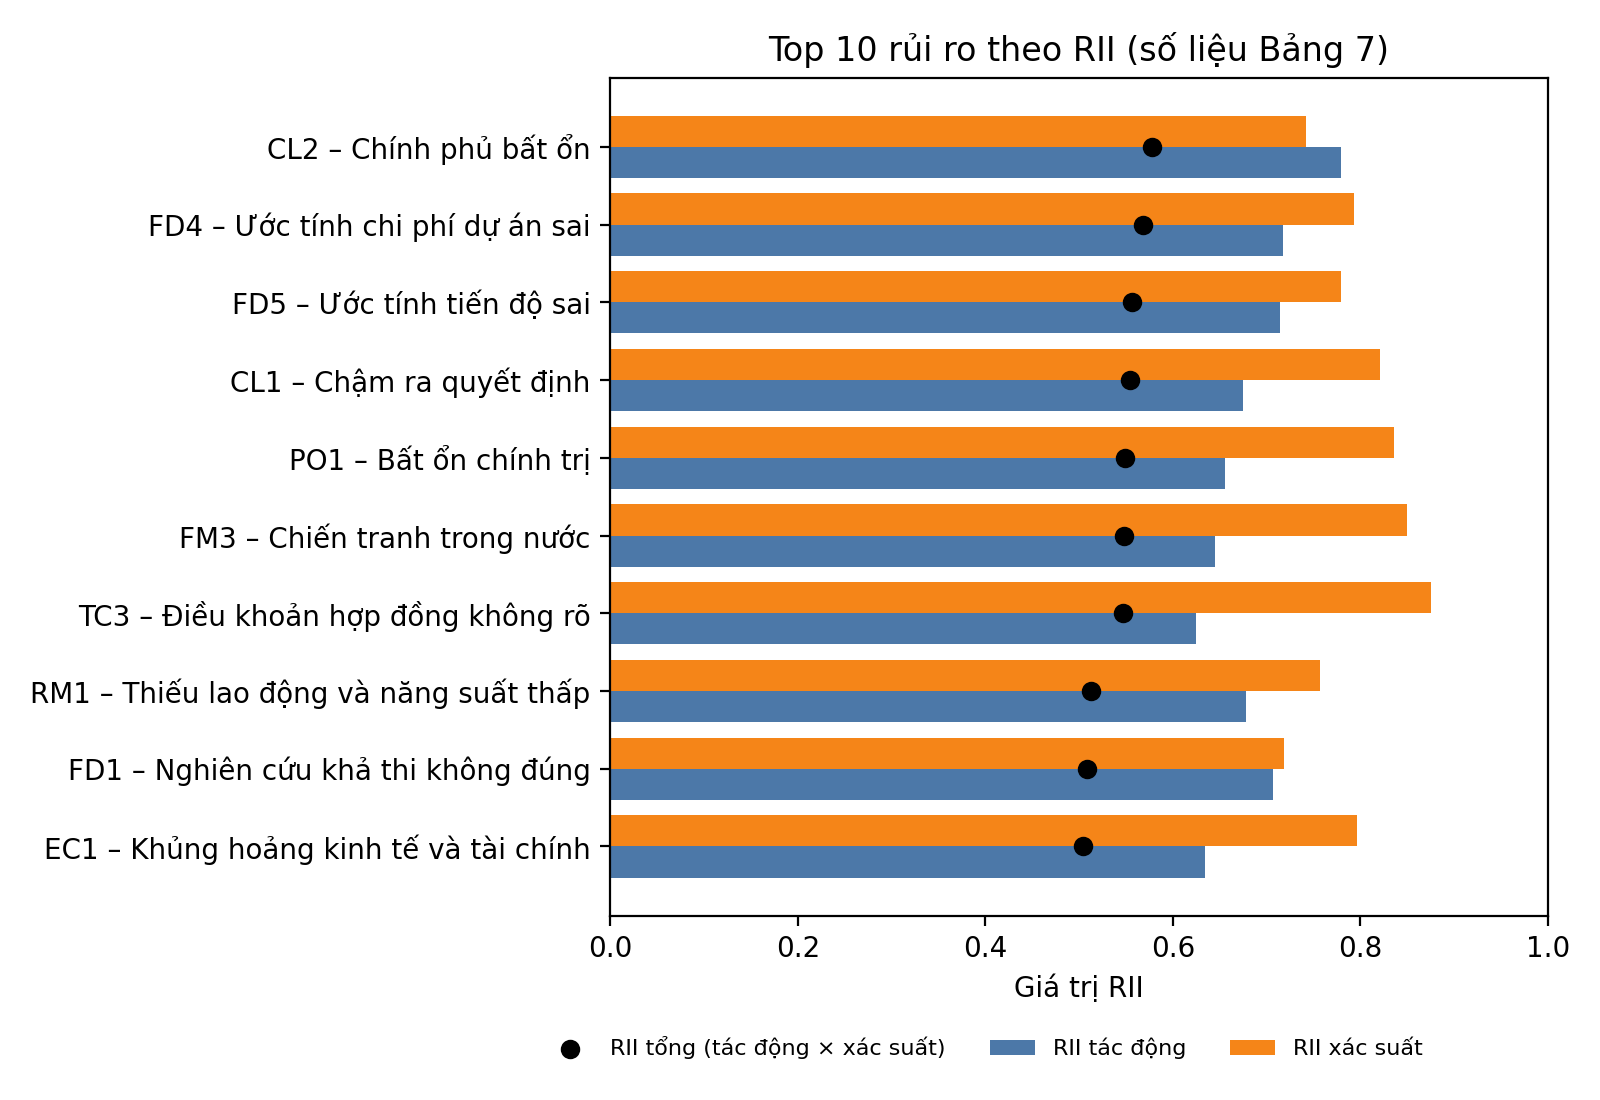
\includegraphics[width=0.85\textwidth]{rii_top10.png}
\caption{RII tác động, RII xác suất và RII tổng của 10 rủi ro hàng đầu (số liệu Bảng 7 trong~\cite{kassem2022})}
\label{fig:rii-top10}
\end{figure}

Ngược lại, ma trận xác suất -- tác động (Bảng 6) \emph{không nhất quán} với RII (Bảng 7). Bài báo không nói cách quy đổi từ điểm sang 5 mức. Nếu dùng cách chia đều thông dụng (mỗi mức rộng 0,2 trên thang RII), thì chỉ 3 trong 6 rủi ro có mặt ở cả hai bảng có mức trùng nhau (Bảng~\ref{tab:pim-rii}). Ví dụ, ``ước tính chi phí sai'' (FD4) có RII tác động 0,717 và RII xác suất 0,793, tức cả hai đều ở mức Cao, nhưng Bảng 6 xếp nó vào ô Rất cao -- Rất cao. Ngoài ra, ``chính phủ bất ổn'' (CL2) đứng đầu theo RII nhưng không có mặt trong top 10 của ma trận.

\begin{table}[H]
\centering
\caption{Mức tác động và xác suất trong Bảng 6 so với mức quy đổi từ RII ở Bảng 7}
\label{tab:pim-rii}
\begin{tabular}{@{}cccccccc@{}}
\toprule
\multirow{2}{*}{\textbf{Mã}} & \multicolumn{2}{c}{\textbf{Bảng 6}} & \multicolumn{2}{c}{\textbf{RII (Bảng 7)}} & \multicolumn{2}{c}{\textbf{Quy đổi}} & \multirow{2}{*}{\textbf{Khớp}} \\
\cmidrule(lr){2-3}\cmidrule(lr){4-5}\cmidrule(lr){6-7}
 & Tác động & Xác suất & Tác động & Xác suất & Tác động & Xác suất & \\
\midrule
FD4 & VH & VH & 0,717 & 0,793 & H & H & Không \\
FD5 & VH & H  & 0,714 & 0,779 & H & H & Không \\
PO1 & H  & VH & 0,656 & 0,836 & H & VH & Có \\
FD1 & H  & VH & 0,707 & 0,718 & H & H & Không \\
CL1 & H  & VH & 0,675 & 0,821 & H & VH & Có \\
RM1 & H  & H  & 0,678 & 0,757 & H & H & Có \\
\bottomrule
\end{tabular}
\end{table}

\subsection{Mô hình đo lường}

\textbf{AVE và CR.} Tính lại AVE và CR của 13 nhóm rủi ro từ 51 loading trong Bảng 8 theo các công thức~\eqref{eq:ave} và~\eqref{eq:cr} cho kết quả khớp hoàn toàn với số bài báo công bố (13/13 nhóm). Riêng biến kết quả EF, năm loading in trong bảng (0,595; 0,761; 0,741; 0,800; 0,591) cho $AVE = 0{,}494$, \emph{dưới} ngưỡng 0,5, trong khi bài báo in 0,549. Tác giả cho biết đã loại câu EF3 (chất lượng kém). Tuy nhiên, thử bỏ lần lượt từng câu thì AVE cao nhất chỉ đạt 0,531 (khi bỏ EF3), không có trường hợp nào bằng 0,549.

\textbf{Fornell--Larcker.} Với ma trận Bảng 9 đã dựng lại, so sánh $\sqrt{AVE}$ của mỗi nhóm với tương quan lớn nhất của nhóm đó cho thấy:
\begin{itemize}
  \item Nhóm \textbf{RM} (nguồn lực và vật tư) \textbf{không đạt}: tương quan với nhóm MR (quản lý dự án) là 0,845, lớn hơn $\sqrt{AVE_{RM}} = 0{,}833$. Bài báo lại kết luận mọi nhóm đều đạt.
  \item Bốn nhóm đạt sát ngưỡng, chênh lệch dưới 0,03: CL (+0,002 so với CO), EC (+0,012 so với PO), PO (+0,019 so với EC), TC (+0,020 so với FD).
  \item Trung bình tương quan giữa các nhóm là 0,712; có 8 trong 78 cặp vượt 0,80.
\end{itemize}
Đây là phát hiện quan trọng nhất của hướng 1, vì chỉ dùng chính số liệu của bài báo. Các nhóm rủi ro chồng lấn nhau nhiều, nhất là cặp RM -- MR và cụm kinh tế -- chính trị -- an ninh. Bài báo không báo cáo HTMT, nên không kiểm tra được mức độ nghiêm trọng của vấn đề này (xem mục~\ref{sec:mo-phong}).

\subsection{Mô hình cấu trúc}

\textbf{Sai số chuẩn của hệ số đường dẫn.} Bảng 11 cho cả $\beta$ và $t$, nên suy ra được sai số chuẩn bootstrap $SE = \beta / t$. Hai đường dẫn bậc 2 (nội bộ và bên ngoài tới EF) có $SE \approx 0{,}064$, là mức hợp lý với cỡ mẫu 314. Nhưng 13 nhóm bậc 1 có $SE$ chỉ từ 0,003 đến 0,006, nhỏ hơn 10 đến 20 lần, dẫn tới các giá trị $t$ rất lớn (26 đến 44). Bài báo không giải thích 13 hệ số này được ước lượng ra sao.

\textbf{$Q^2$.} Tính lại $Q^2 = 1 - SSE/SSO$ từ Bảng 14 khớp cả ba dòng. Bảng 14 không ghi rõ dòng nào ứng với biến nào, nhưng vì $SSO = n \times K$ (mục~\ref{sec:pls-sem}), lấy $SSO$ chia cho 314 sẽ ra số câu hỏi $K$ của biến: 1256/314 = 4 câu (biến EF sau khi bỏ EF3), 6280/314 = 20 câu (rủi ro bên ngoài), 9734/314 = 31 câu (rủi ro nội bộ). Như vậy $Q^2$ của rủi ro nội bộ là 0,527 và bên ngoài là 0,590. Mục 5.3 của bài báo ghi đúng, còn phần Kết luận ghi ngược.

\textbf{GoF.} $\sqrt{0{,}720 \times 0{,}566} = 0{,}638$, khớp với số bài báo công bố. Tuy nhiên, bài báo không nói 0,566 là trung bình AVE của những biến nào. Thử sáu cách lấy trung bình (13 nhóm bậc 1; 13 nhóm và EF; hai nhóm bậc 2; hai nhóm bậc 2 và EF; v.v.) đều không ra 0,566. Theo cách phổ biến nhất (trung bình AVE của các nhóm bậc 1), GoF sẽ xấp xỉ 0,735.

\textbf{Tính nhất quán giữa $R^2$, $\beta$ và $f^2$.} Với hai biến giải thích chuẩn hóa có tương quan $r$, hệ số xác định và hệ số xác định khi bỏ một biến lần lượt là:
\begin{equation}
R^2 = \beta_1^2 + \beta_2^2 + 2\beta_1\beta_2 r, \qquad R^2_{bo\,1} = (\beta_2 + \beta_1 r)^2
\label{eq:r2-hai-bien}
\end{equation}
Lấy $r$ là tương quan giữa trung bình 7 nhóm nội bộ và trung bình 6 nhóm bên ngoài, tính từ ma trận Bảng 9, ta được $r \approx 0{,}831$. Thay $\beta_1 = 0{,}200$ và $\beta_2 = 0{,}673$ vào~\eqref{eq:r2-hai-bien} và~\eqref{eq:f2} được $R^2 = 0{,}717$ (bài báo: 0,720), $f^2_{noi\,bo} = 0{,}044$ (bài báo: 0,042) và $f^2_{ben\,ngoai} = 0{,}494$ (bài báo: 0,471). Vì $r$ chỉ là xấp xỉ (bài báo dùng trọng số PLS chứ không lấy trung bình đều), có thể kết luận phần mô hình cấu trúc bậc 2 \emph{gần như nhất quán} với số liệu tương quan của chính bài báo.

\subsection{Nhận xét}

Phần tính toán cơ bản của bài báo là đúng: RII, AVE và CR của các nhóm, $Q^2$, $R^2$ và $f^2$ của mô hình bậc 2 đều tái hiện được. Các vấn đề tập trung ở bốn chỗ:
\begin{enumerate}
  \item Giá trị phân biệt (Fornell--Larcker không đạt ở nhóm RM).
  \item AVE của biến kết quả.
  \item Cách tính 13 hệ số của các nhóm bậc 1.
  \item Sự không nhất quán giữa ma trận PIM và RII.
\end{enumerate}
Ngoài ra còn các lỗi trình bày như ghi ngược $Q^2$ ở phần Kết luận.

\section{Phân tích trên dữ liệu mô phỏng}
\label{sec:mo-phong}

% Viết sau khi chạy xong bootstrap 5000 lần (results/mo-phong.md)

\section{So sánh và thảo luận}
\label{sec:so-sanh}
